\documentclass[11pt,a4paper]{article}

% ============================================================
%  Paquetes
% ============================================================
\usepackage[utf8]{inputenc}
\usepackage[T1]{fontenc}
\usepackage[spanish,es-tabla,es-nodecimaldot]{babel}
\usepackage{lmodern}
\usepackage[hmargin=2.5cm,vmargin=2.2cm,headsep=14pt]{geometry}
\usepackage{microtype}
\usepackage{amsmath}
\usepackage{booktabs}
\usepackage{tabularx}
\usepackage{float}
\usepackage{graphicx}
\newcommand{\comando}[1]{\par\smallskip{\footnotesize\textit{Comando:} \texttt{#1}}}
\newcommand{\comando}[1]{\par\smallskip{\footnotesize\textit{Comando} -- \texttt{#1}}}
\graphicspath{{../figures/}}

\usepackage[table]{xcolor}
\usepackage{enumitem}
\usepackage[font=small,labelfont=bf,labelsep=period]{caption}
\usepackage{fancyhdr}
\usepackage{tikz}
\usetikzlibrary{arrows.meta,positioning,calc,babel,decorations.pathreplacing}
\usepackage[hidelinks]{hyperref}

\setlist{itemsep=2pt, topsep=4pt}
\setlength{\parskip}{2pt}
\raggedbottom
\setlength{\emergencystretch}{3em}

% Encabezado y pie
\pagestyle{fancy}
\fancyhf{}
\fancyhead[L]{\small CS3014 -- Estructuras de Datos Avanzadas}
\fancyhead[R]{\small Informe final: Skip List vs.\ AVL Tree}
\fancyhead[R]{\small Informe final -- Skip List vs.\ AVL Tree}
\fancyfoot[C]{\small\thepage}
\renewcommand{\headrulewidth}{0.4pt}

% Estilos de las figuras
\tikzset{
  >=Stealth,
  cell/.style={draw, minimum width=6mm, minimum height=4.2mm, inner sep=0pt},
  keycell/.style={cell, font=\small},
  tnode/.style={circle, draw, minimum size=6.5mm, inner sep=0pt, font=\small},
  stepbox/.style={draw, rounded corners=2pt, align=center, font=\small,
                  minimum height=10mm, text width=1.95cm, inner sep=3pt},
}
\newcommand{\on}{\cellcolor{gray!45}}

% ============================================================
\begin{document}

\thispagestyle{empty}
\begin{center}
  {\LARGE\bfseries Skip List frente a AVL Tree}\\[5pt]
  {\large una evaluación experimental sobre conjuntos ordenados dinámicos}\\[14pt]
  {\normalsize Renzo Josimar Felix Aponte \qquad Manyory Estefany Cueva Mendoza}\\[2pt]
  {\normalsize Jefersson Kevin Quicaña Erquinio}\\[6pt]
  {\small Universidad de Ingeniería y Tecnología (UTEC)}\\
  {\small CS3014 -- Estructuras de Datos Avanzadas \quad$\cdot$\quad Noviembre de 2026}
\end{center}
\vspace{2pt}
\noindent\rule{\textwidth}{0.4pt}

\begin{abstract}
\noindent
Implementamos desde cero, en C++17 y con una arquitectura hexagonal, una Skip
List y un AVL Tree, y comparamos experimentalmente su tiempo de búsqueda,
inserción y eliminación con tamaños de entrada entre $10^3$ y $10^6$ y datos en
orden aleatorio, ordenado e inverso. Ambas estructuras tienen costo
$O(\log n)$ (esperado en la skip list, de peor caso en el AVL). En nuestras
mediciones el AVL fue más rápido en las tres operaciones y en todos los
escenarios: con $n = 10^6$ y datos aleatorios, la búsqueda fue unas
$2.6$ veces más rápida y la inserción y la eliminación unas $2$ veces. El
orden de los datos afectó mucho más que la estructura elegida: insertar claves
ordenadas fue hasta $8$ veces más rápido que insertarlas al azar en ambas
estructuras, lo que atribuimos a la localidad de caché. Finalmente, al variar
la probabilidad $p \in \{0.25, 0.50, 0.80\}$ en la Skip List, confirmamos que
$p = 0.50$ ofrece el mejor tiempo en consultas aleatorias, $p = 0.25$ reduce
niveles y memoria a costa de más fallos de caché ($1.2$--$1.5\times$ más lenta
a $n = 10^6$), y $p = 0.80$ degenera hasta ser $51\times$ más lenta que el AVL
en $n = 10^5$ al saturar \texttt{MaxLevel}$\,=20$.
$O(\log n)$ (esperado en la skip list, de peor caso en el AVL). Con $p = 1/2$,
el AVL fue más rápido en las tres operaciones y en todos los escenarios; con
$n = 10^6$ y datos aleatorios, la búsqueda fue unas $2.6$ veces más rápida y la
inserción y la eliminación unas $2$ veces. El orden de los datos afectó mucho
más que la estructura elegida; insertar claves ordenadas fue hasta $8$ veces
más rápido que insertarlas al azar en ambas estructuras, lo que atribuimos a la
localidad de caché. Al variar $p \in \{0.25, 0.50, 0.80\}$ en la Skip List,
vimos que $p = 0.50$ dio el menor tiempo en consultas aleatorias, $p = 0.25$
redujo niveles y memoria a costa de más fallos de caché ($1.2$--$1.5\times$ más
lenta a $n = 10^6$), y $p = 0.80$ degeneró hasta ser $51\times$ más lenta que el
AVL en $n = 10^5$ al saturar \texttt{MaxLevel}$\,=20$.
\end{abstract}
\noindent\rule{\textwidth}{0.4pt}

% ============================================================
\section{Introducción y motivación}

\paragraph{El problema.}
Muchos programas necesitan mantener un conjunto de claves ordenadas que cambia
con el tiempo: se insertan claves nuevas, se buscan claves existentes y se
con el tiempo; se insertan claves nuevas, se buscan claves existentes y se
eliminan otras. Esto aparece, por ejemplo, en el índice de una base de datos o en
el \texttt{std::set} de C++.

\paragraph{Las dos soluciones.}
La solución clásica son los árboles binarios de búsqueda balanceados, como el
AVL Tree, que garantizan $O(\log n)$ por operación en el peor caso a cambio
de aplicar rotaciones para mantenerse balanceados. En 1990, Pugh propuso la
\emph{skip list}~\cite{pugh1990} como alternativa: varias listas enlazadas
ordenadas, una encima de otra, donde la altura de cada nodo se decide al azar.
Así se obtiene $O(\log n)$ esperado sin rotaciones. Según el survey de
\emph{skip list}~\cite{pugh1990} como alternativa, formada por varias listas
enlazadas ordenadas, una encima de otra, donde la altura de cada nodo se decide
al azar. Así se obtiene $O(\log n)$ esperado sin rotaciones. Según el survey de
Xing, Vadrevu y Aref~\cite{vadrevu2024}, hoy la skip list se usa en sistemas
reales como LevelDB, RocksDB, Redis y la clase
\texttt{ConcurrentSkipListMap} de Java.

\paragraph{Por qué compararlas.}
Aunque dos estructuras tengan la misma complejidad asintótica, eso no dice cuál
es más rápida en la práctica. Las constantes ocultas, el número de punteros por nodo,
el uso de la memoria caché o el orden en que llegan los datos pueden cambiar el
tiempo real. Por eso queremos implementar ambas y medirlas bajo las mismas condiciones.


% ============================================================
\section{Conceptos y trabajo relacionado}\label{sec:conceptos}

\subsection{Skip List}

\paragraph{Idea.}
Una skip list está formada por varios niveles. El nivel 1 es una lista enlazada
ordenada con todas las claves. Cada nivel superior contiene solo una parte de
las claves del nivel de abajo y funciona como un ``carril rápido'' que permite
saltar varios nodos de una vez. Una cabecera tiene un puntero por nivel
(Figura~\ref{fig:skiplist}).

\begin{figure}[!htb]
\centering
\begin{tikzpicture}[x=1.25cm, y=4.2mm]
  \foreach \n/\x/\h/\k in {H/0/3/{}, a/1/1/3, b/2/2/5, c/3/1/8, d/4/3/12,
                           e/5/1/15, f/6/2/21, g/7/1/27, N/8/3/{}} {
    \ifx\k\empty\else \node[keycell] (\n-0) at (\x,0) {\k}; \fi
    \foreach \l in {1,...,\h} { \node[cell] (\n-\l) at (\x,\l) {}; }
  }
  \foreach \c in {H-3, d-3, d-2, d-1, e-0} {
    \fill[gray!25] (\c.south west) rectangle (\c.north east);
    \draw (\c.south west) rectangle (\c.north east); }
  \node[font=\small] at (e-0) {15};
  \node[font=\small] at (0,0) {cabecera};
  \node[draw, fill=white, minimum width=6mm, minimum height=12.6mm, font=\small] at (8,2) {NIL};
  \foreach \u/\v/\l in {H/a/1, a/b/1, b/c/1, c/d/1, d/e/1, e/f/1, f/g/1, g/N/1,
                        H/b/2, b/d/2, d/f/2, f/N/2, H/d/3, d/N/3} {
    \fill (\u-\l.center) circle (1.3pt);
    \draw[->] (\u-\l.center) -- (\v-\l.west |- \u-\l.center);
  }
  \foreach \l in {1,2,3} { \node[font=\scriptsize, anchor=west] at (8.35,\l) {nivel \l}; }
  \draw[->, line width=1.3pt] (H-3.center) -- (d-3.west);
  \draw[->, line width=1.3pt] (d-1.center) -- (e-1.west);
\end{tikzpicture}
\caption{Skip list con siete claves y $p = 1/2$. Las celdas sombreadas y los
punteros gruesos muestran la búsqueda de 15: se avanza por el nivel 3 hasta
12; como el siguiente nodo en los niveles 3 y 2 es mayor que 15, se baja hasta
punteros gruesos muestran la búsqueda de 15; se avanza por el nivel 3 hasta
12 y, como el siguiente nodo en los niveles 3 y 2 es mayor que 15, se baja hasta
el nivel 1, donde el siguiente nodo es 15.}
\label{fig:skiplist}
\end{figure}

\paragraph{Operaciones.}
\begin{itemize}
  \item \textbf{Búsqueda:} se empieza en el nivel más alto de la cabecera. En
  \item \textbf{Búsqueda.} Se empieza en el nivel más alto de la cabecera. En
  cada nivel se avanza mientras la siguiente clave sea menor que la buscada; si
  no, se baja un nivel. Se termina en el nivel 1.
  \item \textbf{Inserción:} se busca la posición guardando el último nodo
  \item \textbf{Inserción.} Se busca la posición guardando el último nodo
  visitado en cada nivel. Luego se decide la altura del nuevo nodo lanzando una
  ``moneda'': con probabilidad $p$ sube un nivel más, hasta un máximo
  ``moneda''; con probabilidad $p$ sube un nivel más, hasta un máximo
  \texttt{MaxLevel}. Finalmente se actualizan los punteros de los nodos
  guardados (Figura~\ref{fig:insert}).
  \item \textbf{Eliminación:} se busca la clave de la misma forma y se
  \item \textbf{Eliminación.} Se busca la clave de la misma forma y se
  actualizan los punteros de sus predecesores en cada nivel donde aparece.
\end{itemize}

\begin{figure}[!htb]
\centering
\begin{tikzpicture}[x=1.12cm, y=4.2mm]
  \foreach \n/\x/\h/\k in {H/0/3/{}, a/1/1/3, b/2/2/5, c/3/1/8, d/4/3/12,
                           e/5/1/15, f/7/2/21, g/8/1/27, N/9/3/{}} {
    \ifx\k\empty\else \node[keycell] (\n-0) at (\x,0) {\k}; \fi
    \foreach \l in {1,...,\h} { \node[cell] (\n-\l) at (\x,\l) {}; }
  }
  % nodo nuevo (altura 2)
  \node[keycell, dashed, very thick] (x-0) at (6,0) {17};
  \node[cell, dashed, very thick] (x-1) at (6,1) {};
  \node[cell, dashed, very thick] (x-2) at (6,2) {};
  % predecesores cuyos punteros cambian
  \foreach \c in {d-2, e-1} {
    \fill[gray!25] (\c.south west) rectangle (\c.north east);
    \draw (\c.south west) rectangle (\c.north east); }
  \node[font=\small] at (0,0) {cabecera};
  \node[draw, fill=white, minimum width=6mm, minimum height=12.6mm, font=\small] at (9,2) {NIL};
  \foreach \u/\v/\l in {H/a/1, a/b/1, b/c/1, c/d/1, d/e/1, f/g/1, g/N/1,
                        H/b/2, b/d/2, f/N/2, H/d/3, d/N/3} {
    \fill (\u-\l.center) circle (1.3pt);
    \draw[->] (\u-\l.center) -- (\v-\l.west |- \u-\l.center);
  }
  % punteros nuevos
  \foreach \u/\v/\l in {d/x/2, e/x/1, x/f/1, x/f/2} {
    \fill (\u-\l.center) circle (1.3pt);
    \draw[->, line width=1.3pt] (\u-\l.center) -- (\v-\l.west |- \u-\l.center);
  }
  \node[font=\scriptsize, align=center, above=1mm of x-2] {nuevo nodo\\(altura 2)};
\end{tikzpicture}
\caption{Inserción de 17. La moneda sale ``sube'' una vez y ``no sube'' la
siguiente, así que el nodo tiene altura 2. Solo cambian los punteros de los
predecesores en esos niveles (celdas sombreadas: 12 en el nivel 2 y 15 en el
predecesores en esos niveles (celdas sombreadas, 12 en el nivel 2 y 15 en el
nivel 1); los punteros nuevos se muestran en trazo grueso.}
\label{fig:insert}
\end{figure}

\paragraph{Costo.}
Pugh~\cite{pugh1990} muestra que el número esperado de niveles es del orden de
$\log_{1/p} n$ y que el costo esperado de las tres operaciones es $O(\log n)$.
El número esperado de punteros por nodo es $1/(1-p)$, es decir, 2 cuando
$p = 1/2$, por lo que el espacio esperado es $O(n)$. El peor caso es $O(n)$,
pero tiene una probabilidad muy baja. Además, como la altura de cada nodo se
decide al azar, la forma de la estructura no depende del orden en que llegan
las claves.

\subsection{AVL Tree}

\paragraph{Idea.}
Un AVL Tree~\cite{avl1962} es un árbol binario de búsqueda con una regla extra:
Un AVL Tree~\cite{avl1962} es un árbol binario de búsqueda con una regla extra;
para cada nodo, la diferencia de alturas entre su subárbol izquierdo y el
derecho es como máximo 1. Esa diferencia se llama \emph{factor de balance}.

\paragraph{Operaciones.}
La búsqueda es la misma que en cualquier árbol binario de búsqueda. La
inserción y la eliminación también empiezan igual, pero al terminar se
recorre el camino de vuelta hacia la raíz revisando el factor de balance. Si
algún nodo queda con factor $+2$ o $-2$, se aplica una rotación simple o doble
para recuperar el balance (Figura~\ref{fig:avl}).

\begin{figure}[!htb]
\centering
\begin{tikzpicture}[level distance=9mm, level 1/.style={sibling distance=15mm}]
  \begin{scope}
    \node[tnode] (r) {1}
      child[missing]
      child { node[tnode] {2}
        child[missing]
        child { node[tnode, fill=gray!25] {3} } };
    \node[font=\scriptsize, right=1mm of r] {$+2$};
    \node[font=\small, align=center] at (0.75,-2.75) {después de insertar\\1, 2, 3 (en orden)};
  \end{scope}
  \draw[->, thick] (2.4,-0.9) -- node[above, font=\small] {rotación} (4.1,-0.9);
  \begin{scope}[xshift=5.6cm, yshift=-0.45cm]
    \node[tnode] {2}
      child { node[tnode] {1} }
      child { node[tnode, fill=gray!25] {3} };
    \node[font=\small, align=center] at (0,-2.3) {árbol AVL\\balanceado};
  \end{scope}
\end{tikzpicture}
\caption{Al insertar claves en orden creciente, el AVL pierde el balance en la
raíz (factor $+2$) y lo recupera con una rotación simple a la izquierda.}
\label{fig:avl}
\end{figure}

\paragraph{Costo.}
Gracias a la regla de balance, la altura del árbol es como máximo
aproximadamente $1.44 \log_2(n+2)$~\cite{knuth1998}, así que búsqueda,
inserción y eliminación cuestan $O(\log n)$ en el \emph{peor caso}. Cada nodo
guarda la clave, dos punteros y su altura, por lo que el espacio es $O(n)$. A
diferencia de la skip list, la forma del árbol sí depende del orden en que
llegan las claves, aunque las rotaciones siempre lo mantienen balanceado.

\subsection{Comparación teórica}

La Tabla~\ref{tab:teoria} junta lo que ya se conoce en la literatura. Las dos
estructuras tienen el mismo orden de complejidad, pero una da una garantía
esperada y la otra de peor caso, y mantienen el balance de forma distinta.
La teoría no dice cuál será más rápida en una computadora real, y eso es lo
que queremos medir.

\begin{table}[!htb]
\centering
\begin{tabular}{lcc}
\toprule
\textbf{Aspecto} & \textbf{Skip List} & \textbf{AVL Tree} \\
\midrule
Búsqueda, inserción, eliminación & $O(\log n)$ esperado & $O(\log n)$ peor caso \\
Peor caso de una operación       & $O(n)$ (poco probable) & $O(\log n)$ \\
Espacio                          & $O(n)$ esperado & $O(n)$ \\
Cómo mantiene el balance         & azar (altura aleatoria) & rotaciones \\
¿Depende del orden de los datos? & no & sí (cambian las rotaciones) \\
\bottomrule
\end{tabular}
\caption{Comparación teórica según la literatura~\cite{pugh1990,knuth1998}.}
\label{tab:teoria}
\end{table}

\subsection{Trabajo relacionado}

El trabajo base es el artículo de Pugh~\cite{pugh1990}, que introduce la skip
list, analiza su costo esperado y discute la elección de $p$: recomienda
list, analiza su costo esperado y discute la elección de $p$, recomendando
$p = 1/2$ en general y $p = 1/4$ si se quiere menos variabilidad y menos
memoria. Pugh también reporta comparaciones de tiempo frente a árboles
balanceados, pero con el hardware y los compiladores de 1990, por lo que no
necesariamente representan lo que pasa en una computadora actual.

Como referencia complementaria usamos el survey de Xing, Vadrevu y
Aref~\cite{vadrevu2024}, que revisa muchas variantes de la skip list
(deterministas, concurrentes, orientadas a caché y a memoria externa) y su uso
en bases de datos. Entre las deterministas está la 1-2 skip list de Munro,
Papadakis y Sedgewick~\cite{munro1992}, equivalente a un árbol 2-3. En este
proyecto no implementaremos variantes: nos quedamos con la versión básica de
Pugh.
proyecto no implementamos variantes, sino que nos quedamos con la versión
básica de Pugh.

% ============================================================
\section{Planteamiento del proyecto}\label{sec:plan}

\subsection{Pregunta de investigación}

\begin{quote}
\itshape
¿Cómo se comporta una Skip List frente a un AVL Tree en operaciones de
búsqueda, inserción y eliminación sobre conjuntos ordenados dinámicos?
\end{quote}

Para poder responderla con experimentos, la dividimos en tres preguntas más
concretas:
concretas.
\begin{itemize}
  \item[\textbf{P1.}] ¿Cómo cambia el tiempo de cada operación cuando crece el
  tamaño de la entrada $n$?
  \item[\textbf{P2.}] ¿Influye el orden de los datos (aleatorio, ordenado o
  inverso) en el tiempo de cada estructura?
  \item[\textbf{P3.}] ¿Cómo afecta el parámetro $p$ de la Skip List (que
  controla la altura media de los nodos) a su tiempo real de operación frente
  al AVL?
\end{itemize}

\subsection{Objetivos}

\paragraph{Objetivo general.}
Comparar experimentalmente el tiempo de ejecución de una Skip List y de un AVL
Tree, ambos implementados desde cero, en búsqueda, inserción y eliminación,
bajo distintos tamaños de entrada y órdenes de los datos.

\paragraph{Objetivos específicos.}
\begin{itemize}
  \item[\textbf{O1.}] Implementar una Skip List según el diseño de Pugh~\cite{pugh1990}.
  \item[\textbf{O2.}] Implementar un AVL Tree con inserción y eliminación balanceadas.
  \item[\textbf{O3.}] Verificar la correctitud de ambas implementaciones con
  pruebas automáticas.
  \item[\textbf{O4.}] Construir un generador de datos y un programa de
  medición que apliquen las mismas operaciones a ambas estructuras.
  \item[\textbf{O5.}] Medir, graficar y analizar los tiempos junto con la
  complejidad teórica de cada estructura.
\end{itemize}

% ============================================================
\section{Metodología experimental}\label{sec:metodo}

La Tabla~\ref{tab:diseno} resume el diseño experimental; las subsecciones
siguientes explican cada parte.

\begin{table}[!htb]
\centering
\renewcommand{\arraystretch}{1.2}
\begin{tabularx}{\textwidth}{l X}
\toprule
\textbf{Elemento} & \textbf{Decisión} \\
\midrule
Estructuras   & Skip List ($p \in \{0.25, 0.50, 0.80\}$, \texttt{MaxLevel}$\,=20$) y AVL Tree, ambas en C++17 desde cero \\
Claves        & Enteros de 64 bits, sin duplicados \\
Operaciones   & Inserción, búsqueda (50\,\% claves presentes, 50\,\% ausentes) y eliminación \\
Tamaños       & $n \in \{10^3,\ 10^4,\ 10^5,\ 10^6\}$ \\
Orden de datos& Aleatorio, ordenado (creciente) e inverso (decreciente) \\
Escenarios    & $4 \text{ tamaños} \times 3 \text{ órdenes} = 12$ por estructura \\
Repeticiones  & 10 por escenario, con semillas distintas \\
Métrica       & Tiempo promedio por operación (ns) y desviación estándar \\
Entorno       & Misma máquina y mismas opciones de compilación (\texttt{-O2}) \\
\bottomrule
\end{tabularx}
\caption{Resumen del diseño experimental.}
\label{tab:diseno}
\end{table}

\subsection{Implementación y verificación}

Ambas estructuras tienen la misma interfaz: \texttt{insert(k)},
\texttt{search(k)} y \texttt{remove(k)}. No se usaron librerías externas para
Ambas estructuras tienen la misma interfaz (\texttt{insert(k)},
\texttt{search(k)} y \texttt{remove(k)}). No se usaron librerías externas para
las estructuras, para controlar las condiciones del experimento. Se eligió
$\texttt{MaxLevel} = 20$ porque $\log_2 10^6 \approx 20$ alcanza para el
tamaño máximo con $p = 1/2$. Además del experimento principal con $p = 1/2$, se
evaluó el efecto del parámetro $p$ repitiendo las mediciones con $p = 1/4$
(hasta $n = 10^6$) y $p = 0.80$ (hasta $n = 10^5$) en el experimento E4 (P3).

Antes de medir tiempos se verificó que ambas implementaciones fueran
correctas: se ejecutaron secuencias aleatorias de operaciones y se compararon
correctas; se ejecutaron secuencias aleatorias de operaciones y se compararon
los resultados con \texttt{std::set}, que se usó solo como referencia en las
pruebas y no en las mediciones. También se revisó que el AVL cumpliera su
condición de balance y que cada nivel de la Skip List estuviera ordenado
(Sección~\ref{sec:impl}).

\subsection{Procedimiento de medición}

La Figura~\ref{fig:pipeline} muestra el procedimiento que se aplicó a cada
combinación de tamaño y orden de datos. Todo el procedimiento está automatizado
en el caso de uso \texttt{BenchmarkService} y se ejecuta con un solo comando
(\texttt{./build/benchmark}).

\begin{figure}[!htb]
\centering
\begin{tikzpicture}[node distance=4.5mm]
  \node[stepbox] (gen) {Generar $n$ claves\\(semilla fija)};
  \node[stepbox, right=of gen] (ins) {\textbf{Insertar}\\$n$ claves};
  \node[stepbox, right=of ins] (bus) {\textbf{Buscar}\\$n$ consultas};
  \node[stepbox, right=of bus] (eli) {\textbf{Eliminar}\\$n$ claves};
  \node[stepbox, right=of eli] (rep) {Repetir\\10 veces};
  \node[stepbox, right=of rep] (est) {Promedio y\\gráficos};
  \foreach \u/\v in {gen/ins, ins/bus, bus/eli, eli/rep, rep/est} \draw[->] (\u) -- (\v);
  \draw[->, dashed] (rep.south) -- ++(0,-4mm) -| node[pos=0.25, below, font=\scriptsize] {nuevas semillas} (gen.south);
  \draw[decorate, decoration={brace, amplitude=4pt}]
    ($(ins.north west)+(0,2mm)$) -- ($(eli.north east)+(0,2mm)$)
    node[midway, above=4pt, font=\scriptsize] {se mide el tiempo de cada operación};
\end{tikzpicture}
\caption{Procedimiento experimental para cada tamaño $n$ y orden de datos.
Ambas estructuras reciben exactamente las mismas claves y consultas.}
\label{fig:pipeline}
\end{figure}

Para cada escenario (tamaño $n$ y orden de datos) se siguieron estos pasos:
Para cada escenario (tamaño $n$ y orden de datos) se siguieron estos pasos.
\begin{enumerate}
  \item \textbf{Generación de datos.} \texttt{RandomDatasetGenerator} crea $n$
  claves distintas de 64 bits con un \texttt{std::mt19937\_64} y una semilla
  que depende del escenario y de la repetición. Las claves son pares; luego se
  dejan en orden aleatorio, se ordenan de forma creciente o decreciente. Se
  generan también $n$ consultas: la mitad son claves insertadas elegidas al
  generan también $n$ consultas; la mitad son claves insertadas elegidas al
  azar y la otra mitad son números impares (ausentes con seguridad), todas
  mezcladas en orden aleatorio.
  \item \textbf{Inserción.} Se crea una estructura vacía y se insertan las $n$
  claves en el orden del escenario. Se mide el tiempo del lote completo y se
  divide entre $n$. Al terminar se comprueba que la estructura tenga $n$
  claves y se guarda su altura (AVL) o nivel máximo (Skip List).
  \item \textbf{Búsqueda.} Se ejecutan las $n$ consultas sobre la estructura
  ya construida, midiendo el lote completo. El número de claves encontradas
  se acumula en una variable \texttt{volatile} para que el compilador no
  elimine las búsquedas.
  \item \textbf{Eliminación.} Se eliminan las $n$ claves en el mismo orden de
  la inserción, midiendo el lote completo, y se comprueba que la estructura
  quede vacía.
  \item \textbf{Repetición.} Los pasos 1--4 se repiten 10 veces con semillas
  distintas, más una corrida inicial de calentamiento que se descarta. En
  cada repetición la Skip List y el AVL reciben exactamente el mismo conjunto
  de claves y consultas.
  \item \textbf{Estadísticas.} \texttt{StatisticsCalculator} agrupa las
  mediciones por estructura, operación, $n$ y orden, y calcula la media y la
  desviación estándar muestral. Cada medición se guarda en el archivo
  \texttt{results/raw.csv} y el resumen en \texttt{results/summary.csv};
  luego \texttt{scripts/plot\_results.py} genera los gráficos G1--G4.
\end{enumerate}

Para reducir el ruido, no se imprime nada mientras se mide (el avance se
muestra solo al terminar cada escenario), la generación de datos queda fuera
de la zona medida y el tiempo se toma con
\texttt{std::chrono::steady\_clock} sobre cada lote completo de operaciones,
no sobre operaciones individuales. Todas las corridas se hicieron en la misma
máquina, con el programa compilado con \texttt{-O2}.

\subsection{Presentación de los resultados}

Cada gráfico corresponde a una de las preguntas de la Sección~\ref{sec:plan}
(Tabla~\ref{tab:graficos}). Los gráficos obtenidos se presentan en la
Sección~\ref{sec:resultados}.

\begin{table}[!htb]
\centering
\renewcommand{\arraystretch}{1.2}
\begin{tabularx}{\textwidth}{l l l X}
\toprule
\textbf{Gráfico} & \textbf{Eje $x$} & \textbf{Eje $y$} & \textbf{Qué responde} \\
\midrule
G1: Búsqueda    & $n$ (escala log) & ns por operación & P1 para la búsqueda, Skip List vs.\ AVL \\
G2: Inserción   & $n$ (escala log) & ns por operación & P1 para la inserción, Skip List vs.\ AVL \\
G3: Eliminación & $n$ (escala log) & ns por operación & P1 para la eliminación, Skip List vs.\ AVL \\
G4: Orden       & orden de datos   & ns por operación & P2: efecto del orden con $n = 10^6$ \\
C1--C4: Var.\ $p$ & $n$ / orden      & ns por operación & P3: comparación de $p \in \{0.25, 0.50, 0.80\}$ vs.\ AVL \\
G1 (Búsqueda)    & $n$ (escala log) & ns por operación & P1 para la búsqueda, Skip List vs.\ AVL \\
G2 (Inserción)   & $n$ (escala log) & ns por operación & P1 para la inserción, Skip List vs.\ AVL \\
G3 (Eliminación) & $n$ (escala log) & ns por operación & P1 para la eliminación, Skip List vs.\ AVL \\
G4 (Orden)       & orden de datos   & ns por operación & P2, efecto del orden con $n = 10^6$ \\
C1--C4 (Var.\ $p$) & $n$ / orden      & ns por operación & P3, comparación de $p \in \{0.25, 0.50, 0.80\}$ vs.\ AVL \\
\bottomrule
\end{tabularx}
\caption{Gráficos planeados y la pregunta que responde cada uno.}
\label{tab:graficos}
\end{table}

% ============================================================
\section{Implementación}\label{sec:impl}

\subsection{Arquitectura hexagonal}

El código sigue una arquitectura hexagonal (\emph{puertos y adaptadores}) con
una sola clase por archivo. La idea es que el núcleo del proyecto (las
estructuras y el experimento) no dependa de detalles técnicos como el reloj,
la forma de generar datos o el formato de salida. La
Figura~\ref{fig:hexagonal} muestra las tres capas:
Figura~\ref{fig:hexagonal} muestra las tres capas.

\begin{itemize}
  \item \textbf{Dominio} (\texttt{src/domain}): la interfaz
  \item \textbf{Dominio} (\texttt{src/domain}). Contiene la interfaz
  \texttt{OrderedSet} con \texttt{insert}, \texttt{search} y
  \texttt{remove}, y sus dos implementaciones, \texttt{SkipList} y
  \texttt{AvlTree}, con sus nodos. No depende de nada más.
  \item \textbf{Aplicación} (\texttt{src/application}): el caso de uso
  \item \textbf{Aplicación} (\texttt{src/application}). Incluye el caso de uso
  \texttt{BenchmarkService}, que ejecuta el procedimiento de la
  Figura~\ref{fig:pipeline}, y \texttt{StatisticsCalculator}. Solo conoce
  \emph{puertos} (interfaces): \texttt{OrderedSetFactory},
  \emph{puertos} (interfaces), que son \texttt{OrderedSetFactory},
  \texttt{DatasetGenerator}, \texttt{Timer}, \texttt{ResultRepository} y
  \texttt{ProgressListener}.
  \item \textbf{Infraestructura} (\texttt{src/infrastructure}): los
  \emph{adaptadores} que implementan los puertos:
  \item \textbf{Infraestructura} (\texttt{src/infrastructure}). Agrupa los
  \emph{adaptadores} que implementan los puertos, tales como
  \texttt{SkipListFactory}, \texttt{AvlTreeFactory},
  \texttt{RandomDatasetGenerator}, \texttt{SteadyClockTimer},
  \texttt{CsvResultRepository}, \texttt{ConsoleProgressListener} y el
  \texttt{CommandLineParser}. El archivo \texttt{main.cpp} es la única
  pieza que conecta todo.
  \texttt{CsvResultRepository}, \texttt{ConsoleProgressListener} y
  \texttt{CommandLineParser}. El archivo \texttt{main.cpp} es la única pieza
  que conecta todo.
\end{itemize}

Gracias a esto, agregar una estructura nueva (por ejemplo, un árbol
rojo-negro) solo requiere implementar \texttt{OrderedSet} y una fábrica, sin
tocar el caso de uso; y cambiar el formato de salida solo requiere otro
\texttt{ResultRepository}.

\begin{figure}[!htb]
\centering
\begin{tikzpicture}[
  box/.style={draw, rounded corners=2pt, align=center, font=\small, inner sep=4pt},
  port/.style={box, fill=gray!12, font=\scriptsize}]
  \node[box, minimum width=5.6cm, minimum height=1.2cm, fill=gray!30, inner sep=6pt] (dom)
    {\textbf{Dominio}\\ \texttt{OrderedSet}, \texttt{SkipList}, \texttt{AvlTree}};
  \node[box, minimum width=13.5cm, minimum height=3.6cm, anchor=center] (app) at (dom) {};
  \node[font=\small, anchor=north] at (app.north) {\textbf{Aplicación}: \texttt{BenchmarkService}, \texttt{StatisticsCalculator}};
  \node[font=\small, anchor=north] at (app.north) {\textbf{Aplicación} -- \texttt{BenchmarkService}, \texttt{StatisticsCalculator}};
  \node[port, anchor=west] (p1) at ($(app.west)+(0.15,0.6)$) {\texttt{OrderedSetFactory}};
  \node[port, anchor=west] (p2) at ($(app.west)+(0.15,-0.6)$) {\texttt{DatasetGenerator}};
  \node[port, anchor=east] (p3) at ($(app.east)+(-0.15,0.6)$) {\texttt{Timer}};
  \node[port, anchor=east] (p4) at ($(app.east)+(-0.15,-0.1)$) {\texttt{ResultRepository}};
  \node[port, anchor=east] (p5) at ($(app.east)+(-0.15,-0.8)$) {\texttt{ProgressListener}};
  \node[box, below=6mm of app, text width=13cm, font=\scriptsize] (inf)
    {\textbf{Infraestructura (adaptadores):} \texttt{SkipListFactory}, \texttt{AvlTreeFactory},
    {\textbf{Infraestructura (adaptadores)} -- \texttt{SkipListFactory}, \texttt{AvlTreeFactory},
     \texttt{RandomDatasetGenerator}, \texttt{SteadyClockTimer}, \texttt{CsvResultRepository},
     \texttt{ConsoleProgressListener}, \texttt{CommandLineParser}, \texttt{main.cpp}};
  \draw[->, dashed] (inf.north) -- node[right, font=\scriptsize] {implementan los puertos} (app.south);
\end{tikzpicture}
\caption{Arquitectura hexagonal del proyecto. Las dependencias apuntan hacia
adentro: la infraestructura conoce a la aplicación y al dominio, pero no al
adentro; la infraestructura conoce a la aplicación y al dominio, pero no al
revés.}
\label{fig:hexagonal}
\end{figure}

\subsection{Detalles de las estructuras}

La \textbf{Skip List} sigue a Pugh~\cite{pugh1990}: una cabecera con
\texttt{MaxLevel}$=20$ punteros, nodos con un vector de punteros
La \textbf{Skip List} sigue el diseño de Pugh~\cite{pugh1990}, con una cabecera
de \texttt{MaxLevel}$=20$ punteros, nodos con un vector de punteros
\texttt{forward}, altura aleatoria con un \texttt{std::mt19937\_64} con semilla
y un buffer \texttt{update} reutilizable para no reservar memoria en cada
operación. Al eliminar se reduce el nivel activo si los niveles superiores
quedan vacíos.

El \textbf{AVL Tree} usa inserción y eliminación recursivas que devuelven la
nueva raíz del subárbol y llaman a \texttt{rebalance} al volver; este método
actualiza la altura y aplica las rotaciones simples o dobles (casos LL, RR, LR
y RL). Para eliminar un nodo con dos hijos se usa su sucesor, extraído con
\texttt{removeMin}.

Las claves se generan como enteros de 64 bits distintos; las claves
insertadas son pares y las consultas ausentes son impares, así el 50\,\% de
las búsquedas falla con seguridad sin tener que comprobarlo.

\subsection{Verificación}

El programa \texttt{correctness\_tests} prueba ambas estructuras (y la skip
list también con $p = 1/4$) con casos borde (estructura vacía, duplicados),
entradas ordenadas e inversas, y 10 secuencias de 50\,000 operaciones
aleatorias comparadas una por una con \texttt{std::set}. Además, cada cierto
número de operaciones se llama a \texttt{checkInvariants()}: en el AVL revisa
el orden de búsqueda, el factor de balance y las alturas guardadas; en la
skip list revisa que cada nivel esté ordenado y sea sublista del nivel de
número de operaciones se llama a \texttt{checkInvariants()}; en el AVL revisa
el orden de búsqueda, el factor de balance y las alturas guardadas, mientras que
en la skip list revisa que cada nivel esté ordenado y sea sublista del nivel de
abajo. También se comprueba la cota de altura
$h \le 1.44 \log_2(n+2)$ del AVL. Todas las pruebas pasaron.

% ============================================================
\section{Resultados}\label{sec:resultados}

Los experimentos se ejecutaron en una laptop con un AMD Ryzen 5 8645HS (6
núcleos, 12 hilos) y 16\,GB de RAM, con Windows 11 y GCC 13.1 (\texttt{-O2}).
La Tabla~\ref{tab:experimentos} lista los cuatro experimentos realizados, qué
objetivo y pregunta cubre cada uno y su resultado principal. Las subsecciones
siguientes presentan cada experimento.

\begin{table}[!htb]
\centering
\renewcommand{\arraystretch}{1.2}
\small
\begin{tabularx}{\textwidth}{l >{\raggedright\arraybackslash}p{3.6cm} l >{\raggedright\arraybackslash}X}
\toprule
\textbf{Exp.} & \textbf{Qué se hizo} & \textbf{Cubre} & \textbf{Resultado principal} \\
\midrule
E1 & Pruebas de correctitud contra \texttt{std::set} e invariantes
   & O1, O2, O3 & 3 configuraciones, 10 secuencias de 50\,000 operaciones cada una: 0 fallos \\
   & O1, O2, O3 & 3 configuraciones, 10 secuencias de 50\,000 operaciones cada una, con 0 fallos \\
E2 & Tiempo vs.\ tamaño $n$ ($10^3$--$10^6$), 3 operaciones, 10 repeticiones
   & O4, O5, P1 & AVL más rápido en todos los casos; ventaja de 1.1 a 2.9$\times$, mayor con $n$ grande \\
E3 & Tiempo vs.\ orden de los datos con $n=10^6$
   & O4, O5, P2 & El orden pesa más que la estructura: datos ordenados hasta 10$\times$ más rápidos \\
   & O4, O5, P2 & El orden pesa más que la estructura; datos ordenados hasta 10$\times$ más rápidos \\
E4 & Variación de $p \in \{0.25, 0.50, 0.80\}$ (10 repeticiones)
   & O5, P3 & $p=0.25$ ahorra niveles pero es 1.2--1.5$\times$ más lenta en aleatorio; $p=0.80$ degenera (51$\times$ vs.\ AVL a $10^5$) \\
\bottomrule
\end{tabularx}
\caption{Experimentos realizados y su relación con los objetivos (O1--O5) y
las preguntas (P1--P3) de la Sección~\ref{sec:plan}.}
\label{tab:experimentos}
\end{table}

\subsection{E1: verificación de correctitud}
\subsection{E1 -- Verificación de correctitud}

Antes de medir tiempos se ejecutó \texttt{correctness\_tests} sobre tres
configuraciones: Skip List con $p=1/2$, Skip List con $p=1/4$ y AVL. Para cada
configuraciones (Skip List con $p=1/2$, Skip List con $p=1/4$ y AVL). Para cada
una se probaron casos borde (vacío, duplicados, eliminar una clave
inexistente), inserción de 5\,000 claves crecientes y decrecientes seguida de
la eliminación de la mitad, y 10 secuencias de 50\,000 operaciones aleatorias
(5 con claves en $[-500, 500]$, con muchas repeticiones, y 5 en
$[-10^6, 10^6]$). Cada resultado de \texttt{insert}, \texttt{search} y
\texttt{remove} se comparó con \texttt{std::set} y cada 1\,000 operaciones se
verificaron los invariantes. Además, tras insertar $10^5$ claves en orden en el
AVL se comprobó que su altura no supere $1.44\log_2(n+2)$. Las
\textbf{1\,500\,000 operaciones} verificadas dieron \textbf{0 fallos}, con lo
que se dan por cumplidos O1, O2 y O3.

\begin{table}[!htb]
\centering
\renewcommand{\arraystretch}{1.15}
\small
\begin{tabular}{lccccr}
\toprule
\textbf{Estructura} & \textbf{Casos} & \textbf{Entradas} & \textbf{Aleatorias vs.} & \textbf{Compro-} & \textbf{Fallos} \\
 & \textbf{borde} & \textbf{ordenadas} & \texttt{\textbf{std::set}} & \textbf{baciones} & \\
\midrule
Skip List $p=1/2$ & OK & OK & OK & 585\,815 & 0 \\
Skip List $p=1/4$ & OK & OK & OK & 585\,815 & 0 \\
AVL Tree          & OK & OK & OK & 585\,815 & 0 \\
\midrule
AVL: $h \le 1.44\log_2(n+2)$ & \multicolumn{4}{c}{OK ($n = 10^5$ claves en orden)} & 0 \\
AVL ($h \le 1.44\log_2(n+2)$) & \multicolumn{4}{c}{OK ($n = 10^5$ claves en orden)} & 0 \\
\bottomrule
\end{tabular}
\comando{./build/correctness\_tests}
\caption{E1: resultado de las pruebas de correctitud.}
\caption{E1 -- Resultado de las pruebas de correctitud.}
\label{tab:e1}
\end{table}

\begin{figure}[!htb]
\centering
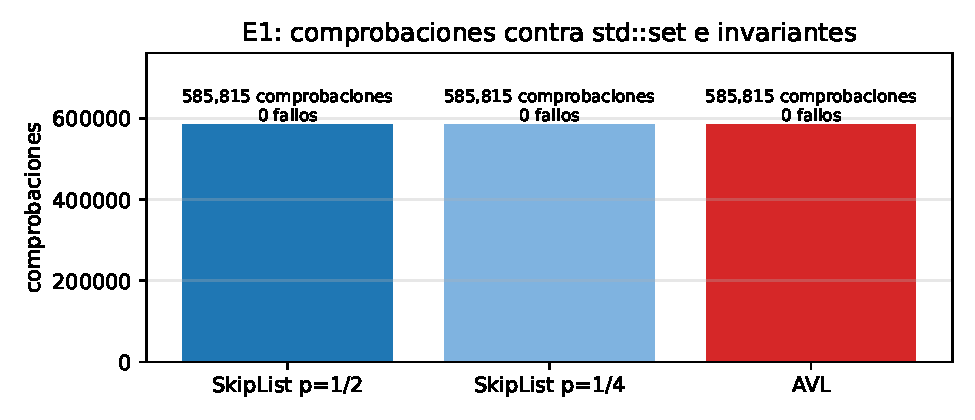
\includegraphics[width=0.75\textwidth]{e1_correctitud.pdf}
\caption{E1: comprobaciones realizadas por estructura y fallos encontrados.}
\caption{E1 -- Comprobaciones realizadas por estructura y fallos encontrados.}
\label{fig:e1}
\end{figure}


El programa de medición también comprueba la correctitud durante E2--E4: tras
El programa de medición también comprueba la correctitud durante E2--E4; tras
insertar verifica que la estructura tenga exactamente $n$ claves, y tras
eliminar, que quede vacía. Ninguna corrida falló estas comprobaciones.

\subsection{E2 y E3: tiempos de ejecución}
\subsection{E2 y E3 -- Tiempos de ejecución}

Se corrieron los 12 escenarios con 10 repeticiones cada uno, más una corrida
de calentamiento descartada; el experimento completo tardó unos 3 minutos. Las
barras de error de los gráficos son la desviación estándar entre
repeticiones. La Tabla~\ref{tab:res1e6} resume los valores para $n = 10^6$ y
la Tabla~\ref{tab:busqueda} los de las tres operaciones con datos aleatorios para todos
los tamaños.

\begin{table}[!htb]
\centering
\renewcommand{\arraystretch}{1.15}
\small
\begin{tabular}{r rr rr rr c}
\toprule
& \multicolumn{2}{c}{\textbf{Búsqueda (ns)}} & \multicolumn{2}{c}{\textbf{Inserción (ns)}} & \multicolumn{2}{c}{\textbf{Eliminación (ns)}} & \textbf{Altura} \\
\cmidrule(lr){2-3}\cmidrule(lr){4-5}\cmidrule(lr){6-7}
$n$ & SL & AVL & SL & AVL & SL & AVL & AVL / SL \\
\midrule
$10^3$ & 64   & 42  & 160  & 96  & 99   & 77  & 12 / 11 \\
$10^4$ & 133  & 70  & 220  & 153 & 160  & 114 & 16 / 15 \\
$10^5$ & 445  & 155 & 443  & 253 & 391  & 220 & 20 / 18 \\
$10^6$ & 1859 & 703 & 1861 & 934 & 1739 & 903 & 24 / 20 \\
\bottomrule
\end{tabular}
\comando{./build/benchmark -{}-out results \&\& python scripts/plot\_results.py}
\caption{E2: tiempo promedio por operación según $n$, con datos en orden
\caption{E2 -- Tiempo promedio por operación según $n$, con datos en orden
aleatorio (SL = Skip List, $p=1/2$). Las desviaciones estándar están en
\texttt{results/summary.csv} y como barras de error en G1--G3.}
\label{tab:busqueda}
\end{table}

\begin{table}[!htb]
\centering
\renewcommand{\arraystretch}{1.15}
\begin{tabular}{llrrr}
\toprule
\textbf{Orden} & \textbf{Operación} & \textbf{Skip List (ns)} & \textbf{AVL (ns)} & \textbf{SL / AVL} \\
\midrule
Aleatorio & Búsqueda    & $1859 \pm 197$ & $703 \pm 42$ & 2.6 \\
          & Inserción   & $1861 \pm 137$ & $934 \pm 54$ & 2.0 \\
          & Eliminación & $1739 \pm 101$ & $903 \pm 47$ & 1.9 \\
\midrule
Ordenado  & Búsqueda    & $1365 \pm 164$ & $580 \pm 70$ & 2.4 \\
          & Inserción   & $185 \pm 51$   & $110 \pm 26$ & 1.7 \\
          & Eliminación & $98 \pm 16$    & $84 \pm 15$  & 1.2 \\
\midrule
Inverso   & Búsqueda    & $1566 \pm 159$ & $683 \pm 39$ & 2.3 \\
          & Inserción   & $145 \pm 16$   & $137 \pm 19$ & 1.1 \\
          & Eliminación & $191 \pm 21$   & $107 \pm 3$  & 1.8 \\
\bottomrule
\end{tabular}
\comando{./build/benchmark -{}-out results}
\caption{E3: tiempo promedio por operación (media $\pm$ desviación estándar) con
\caption{E3 -- Tiempo promedio por operación (media $\pm$ desviación estándar) con
$n = 10^6$ en los tres órdenes de datos.}
\label{tab:res1e6}
\end{table}

\begin{figure}[!htb]
\centering
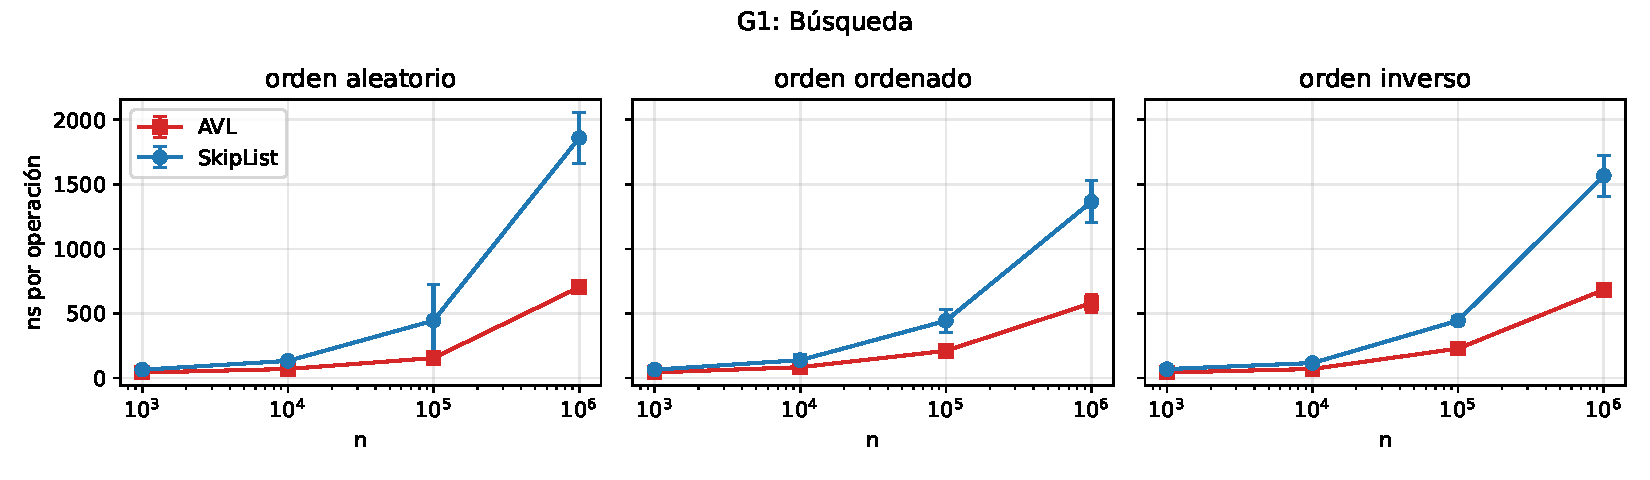
\includegraphics[width=\textwidth]{g1_search.pdf}
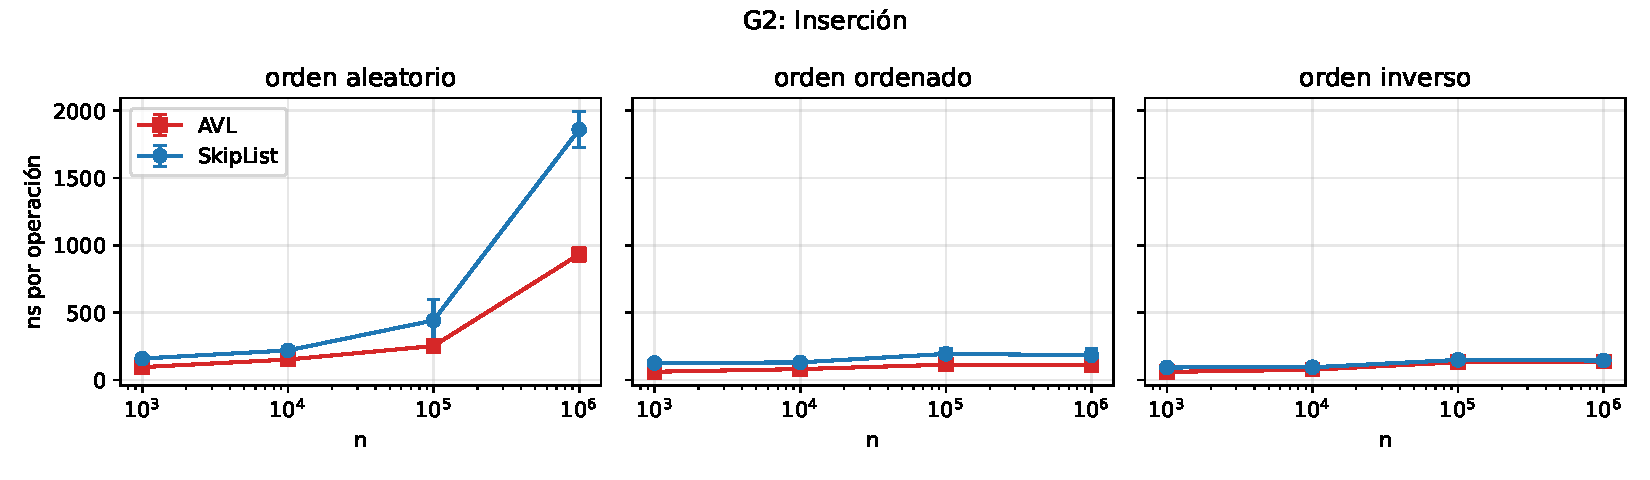
\includegraphics[width=\textwidth]{g2_insert.pdf}
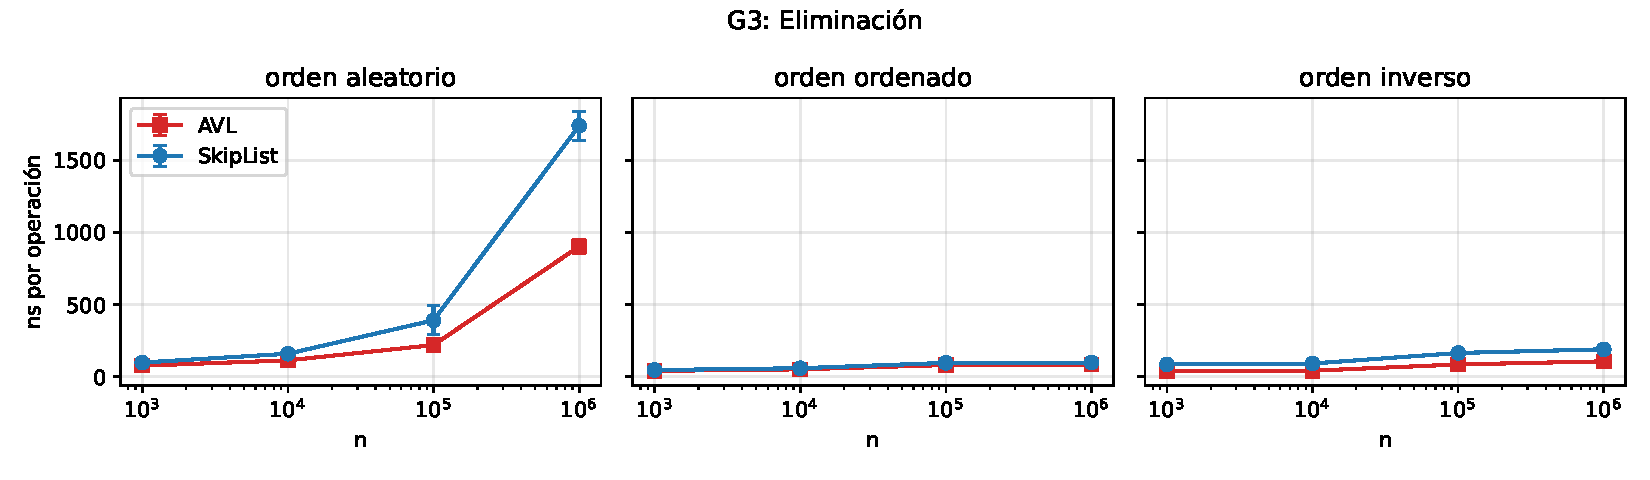
\includegraphics[width=\textwidth]{g3_remove.pdf}
\comando{python scripts/plot\_results.py results/summary.csv figures}
\caption{G1--G3: tiempo por operación en función de $n$ (escala logarítmica)
\caption{G1--G3 -- Tiempo por operación en función de $n$ (escala logarítmica)
para cada orden de datos.}
\label{fig:g123}
\end{figure}

\begin{figure}[!htb]
\centering
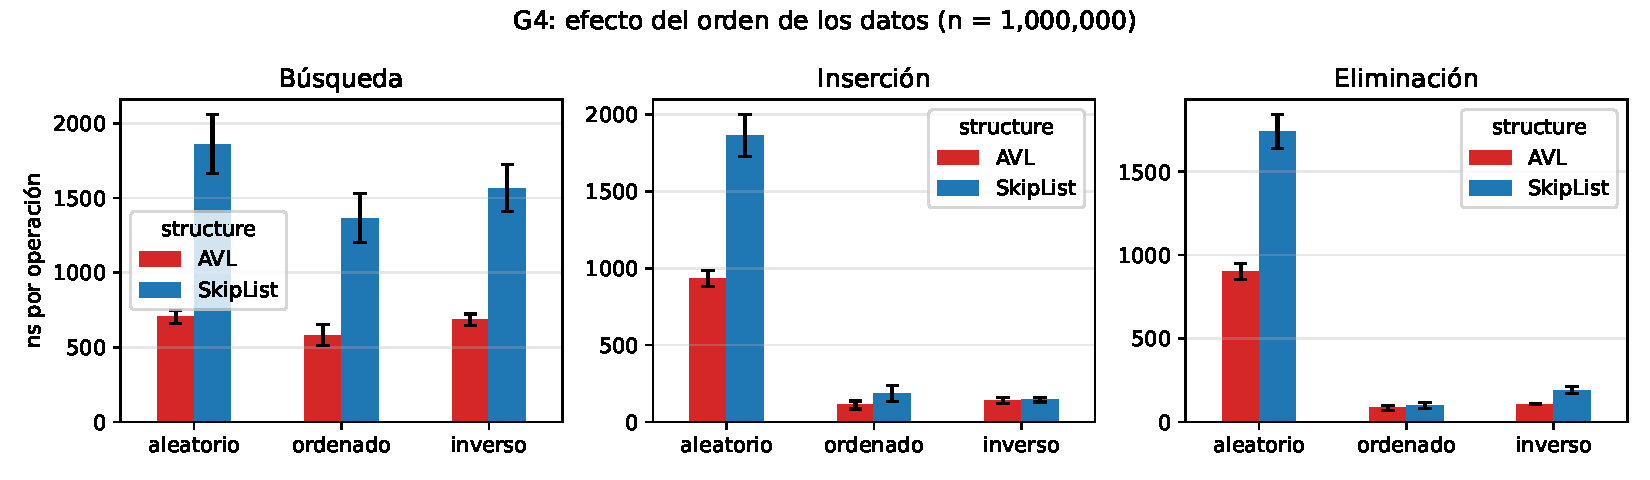
\includegraphics[width=\textwidth]{g4_orden.pdf}
\comando{python scripts/plot\_results.py results/summary.csv figures}
\caption{G4: efecto del orden de los datos con $n = 10^6$.}
\caption{G4 -- Efecto del orden de los datos con $n = 10^6$.}
\label{fig:g4}
\end{figure}

\subsubsection*{E2 (P1): efecto del tamaño de la entrada}
\subsubsection*{E2 (P1) -- Efecto del tamaño de la entrada}

En las tres operaciones (Figura~\ref{fig:g123}) el AVL es más rápido que la
skip list para todos los tamaños. Con $n = 10^3$ la diferencia es pequeña
(por ejemplo, 42\,ns frente a 64\,ns en la búsqueda), pero crece con $n$: con
(por ejemplo, 42\,ns frente a 64\,ns en la búsqueda), pero crece con $n$; con
datos aleatorios la búsqueda pasa de ser 1.5 veces más lenta en la skip list
con $n=10^3$ a 2.6 veces con $n=10^6$.

Si el costo fuera solo $O(\log n)$, el tiempo debería crecer de forma lineal
en un eje logarítmico. Hasta $n = 10^4$ ocurre más o menos así, pero entre
$10^5$ y $10^6$ el tiempo sube mucho más rápido (la búsqueda en el AVL pasa
de 155 a 703\,ns). Esto coincide con el momento en que la estructura deja de
caber en la caché del procesador: con $10^6$ nodos se ocupan decenas de
caber en la caché del procesador; con $10^6$ nodos se ocupan decenas de
megabytes, y cada paso de la búsqueda pasa a ser un acceso a memoria
principal. La skip list sufre más este efecto porque recorre más nodos por
búsqueda (en promedio unos $2\log_2 n$ comparaciones con $p=1/2$, frente a
$\approx\log_2 n$ del AVL) y porque cada nodo guarda sus punteros en un vector
aparte, lo que agrega un acceso indirecto más por nodo visitado.

\subsubsection*{E3 (P2): efecto del orden de los datos}
\subsubsection*{E3 (P2) -- Efecto del orden de los datos}

El orden de los datos tuvo un efecto mucho mayor que la estructura elegida
(Figura~\ref{fig:g4}). Con $n=10^6$, insertar claves ordenadas fue unas 8
veces más rápido que insertarlas al azar en el AVL (110 frente a 934\,ns) y
unas 10 veces en la skip list (185 frente a 1861\,ns). Con claves ordenadas
cada inserción recorre casi el mismo camino que la anterior, que ya está en
caché; con claves aleatorias cada inserción toca un camino distinto. La
búsqueda, en cambio, casi no depende del orden de inserción, porque las
consultas siempre se hacen en orden aleatorio.

La teoría también se confirma en la forma de las estructuras: la altura del
La teoría también se confirma en la forma de las estructuras; la altura del
AVL sí depende del orden (24 con datos aleatorios y 20 con datos ordenados,
por debajo de la cota $1.44\log_2(n+2)\approx 28.7$), mientras que el nivel
máximo de la skip list fue de unos 20 en los tres casos, porque solo depende
de la moneda y no de las claves.

\subsection{E4 (P3): efecto del parámetro \texorpdfstring{$p$}{p} en la Skip List}\label{sec:e4}\label{sec:p3}
\subsection{E4 (P3) -- Efecto del parámetro \texorpdfstring{$p$}{p} en la Skip List}\label{sec:e4}\label{sec:p3}

\paragraph{Motivación y configuración.}
Pugh~\cite{pugh1990} recomienda $p=1/2$ como valor general y $p=1/4$ cuando se
busca menor uso de memoria (en promedio $1/(1-p) \approx 1.33$ punteros por
nodo frente a 2). Con $p$ alto (cerca de 1), demasiados nodos suben a niveles
superiores y los ``carriles rápidos'' pierden eficacia; con $p$ bajo hay menos
niveles pero se recorren más nodos horizontales antes de bajar. Para responder
\textbf{P3} en igualdad de condiciones (misma máquina y 10 repeticiones con las
mismas semillas) repetimos los experimentos usando el parámetro \texttt{-{}-p}
para $p \in \{0.25, 0.50, 0.80\}$:
\begin{itemize}
  \item $p = 0.50$ y $p = 0.25$: $n \in \{10^3, 10^4, 10^5, 10^6\}$, 10 repeticiones (\texttt{results/} y \texttt{results/p025/}).
  \item $p = 0.80$: $n \in \{10^3, 10^4, 10^5\}$, 10 repeticiones (\texttt{results/p080/}); se omitió $n = 10^6$ porque con \texttt{MaxLevel}$\,=20$ la estructura degenera y los tiempos crecen de forma casi lineal.
\end{itemize}
quiere usar menos memoria (en promedio $1/(1-p) \approx 1.33$ punteros por nodo
en lugar de 2). Si $p$ es muy alto, demasiados nodos suben a los niveles
superiores y los ``carriles rápidos'' dejan de saltar elementos; si $p$ es bajo,
hay menos niveles pero se recorren más nodos horizontales antes de bajar. Para
responder \textbf{P3} bajo las mismas condiciones (misma máquina, 10
repeticiones y mismas semillas) repetimos los experimentos cambiando solo la
opción \texttt{-{}-p} para $p \in \{0.25, 0.50, 0.80\}$. Con $p = 0.50$ y
$p = 0.25$ medimos desde $n = 10^3$ hasta $n = 10^6$ (\texttt{results/} y
\texttt{results/p025/}), mientras que con $p = 0.80$ medimos hasta $n = 10^5$
(\texttt{results/p080/}), ya que con \texttt{MaxLevel}$\,=20$ la estructura
degenera y en $n = 10^6$ el tiempo crece de forma casi lineal.

\paragraph{Comparación a $n = 10^6$ ($p=1/2$ vs.\ $p=1/4$ vs.\ AVL).}
La Tabla~\ref{tab:p025} y la Figura~\ref{fig:e4} comparan $p=1/2$ y $p=1/4$
frente al AVL en el tamaño máximo con datos aleatorios.
frente al AVL en $n = 10^6$ con datos aleatorios.

\begin{table}[!htb]
\centering
\renewcommand{\arraystretch}{1.15}
\begin{tabular}{lrrr}
\toprule
\textbf{Operación} & \textbf{$p=1/2$ (ns)} & \textbf{$p=1/4$ (ns)} & \textbf{AVL (ns)} \\
\midrule
Búsqueda    & $1859 \pm 197$ & $2748 \pm 225$ & $\mathbf{703 \pm 42}$ \\
Inserción   & $1861 \pm 137$ & $2419 \pm 304$ & $\mathbf{934 \pm 54}$ \\
Eliminación & $1739 \pm 101$ & $2322 \pm 307$ & $\mathbf{903 \pm 47}$ \\
Nivel máximo / altura & 19.5 & 10.7 & 24 \\
\bottomrule
\end{tabular}
\comando{./build/benchmark -{}-p 0.25 -{}-out results/p025 \&\& python scripts/plot\_extra.py}
\caption{E4: Skip List con $p=1/2$ y $p=1/4$ frente al AVL ($n=10^6$, orden aleatorio, 10 repeticiones).}
\caption{E4 -- Skip List con $p=1/2$ y $p=1/4$ frente al AVL ($n=10^6$, orden aleatorio, 10 repeticiones).}
\label{tab:p025}
\end{table}

\begin{figure}[!htb]
\centering
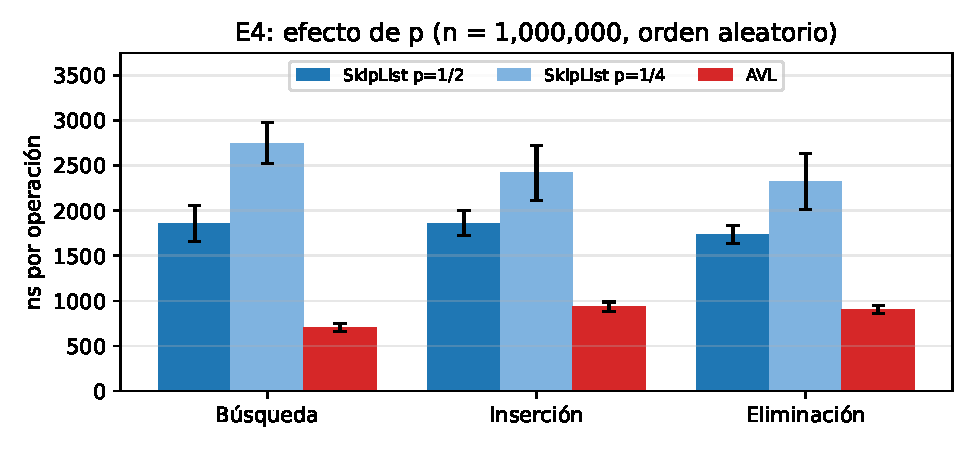
\includegraphics[width=0.75\textwidth]{e4_p025.pdf}
\caption{E4: comparación de la Skip List con $p=1/2$ y $p=1/4$ y el AVL ($n = 10^6$, orden aleatorio).}
\caption{E4 -- Comparación de la Skip List con $p=1/2$ y $p=1/4$ y el AVL ($n = 10^6$, orden aleatorio).}
\label{fig:e4}
\end{figure}

\paragraph{Comparación de las cuatro series ($p \in \{0.25, 0.50, 0.80\}$ y AVL).}
La Tabla~\ref{tab:resp3} muestra los tiempos medios a $n = 10^5$ (máximo común
a las cuatro series) y las Figuras~\ref{fig:c123} y~\ref{fig:c4} presentan la
evolución con $n$ y el efecto del orden de los datos.
La Tabla~\ref{tab:resp3} reúne los tiempos de las cuatro configuraciones en
$n = 10^5$ (el mayor tamaño común a todas), y las Figuras~\ref{fig:c123}
y~\ref{fig:c4} muestran su evolución con $n$ y con el orden de los datos.

\begin{table}[!htb]
\centering
\small
\renewcommand{\arraystretch}{1.15}
\begin{tabular}{llrrrr}
\toprule
\textbf{Orden} & \textbf{Operación} &
\textbf{AVL} & \textbf{SL $p{=}0.25$} & \textbf{SL $p{=}0.50$} & \textbf{SL $p{=}0.80$} \\
\multicolumn{2}{l}{\small(ns por operación, $n=10^5$, 10 reps)} & & & & \\
\midrule
Aleatorio & Búsqueda    & \textbf{155} &  656 &  445 & 7\,878 \\
          & Inserción   & \textbf{253} &  481 &  443 & 3\,827 \\
          & Eliminación & \textbf{220} &  476 &  391 & 3\,790 \\
\midrule
Ordenado  & Búsqueda    & \textbf{210} &  565 &  443 & 6\,167 \\
          & Inserción   & \textbf{115} &  174 &  195 & 5\,861 \\
          & Eliminación &  82          & \textbf{64} &   96 &    86 \\
\midrule
Inverso   & Búsqueda    & \textbf{228} &  538 &  445 & 5\,965 \\
          & Inserción   & 133          & \textbf{107} &  150 &   146 \\
          & Eliminación & \textbf{86}  &  131 &  165 & 5\,709 \\
\bottomrule
\end{tabular}
\comando{./build/benchmark -{}-p 0.80 -{}-sizes 1000,10000,100000 -{}-out results/p080 \&\& python scripts/plot\_p\_experiment.py}
\caption{E4 (P3): tiempo medio por operación (ns) con $n = 10^5$ para las cuatro
configuraciones en la misma máquina (10 repeticiones). Los valores más bajos de
cada fila aparecen en negrita.}
\caption{E4 (P3) -- Tiempo medio por operación (ns) con $n = 10^5$ para las
cuatro configuraciones en la misma máquina (10 repeticiones). Los valores más
bajos de cada fila aparecen en negrita.}
\label{tab:resp3}
\end{table}

\begin{figure}[!htb]
\centering
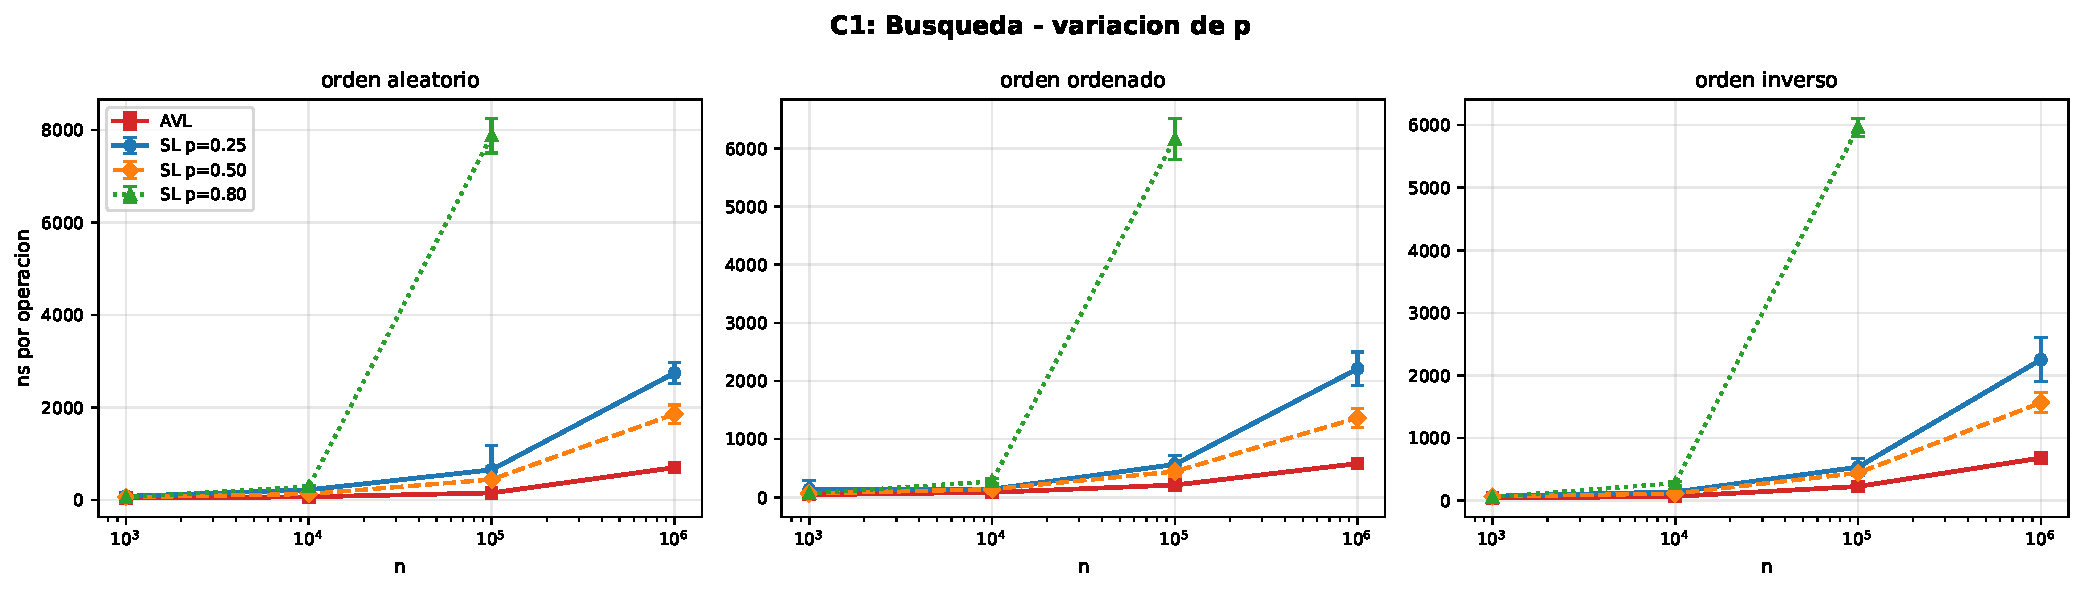
\includegraphics[width=\textwidth]{c1_search.pdf}
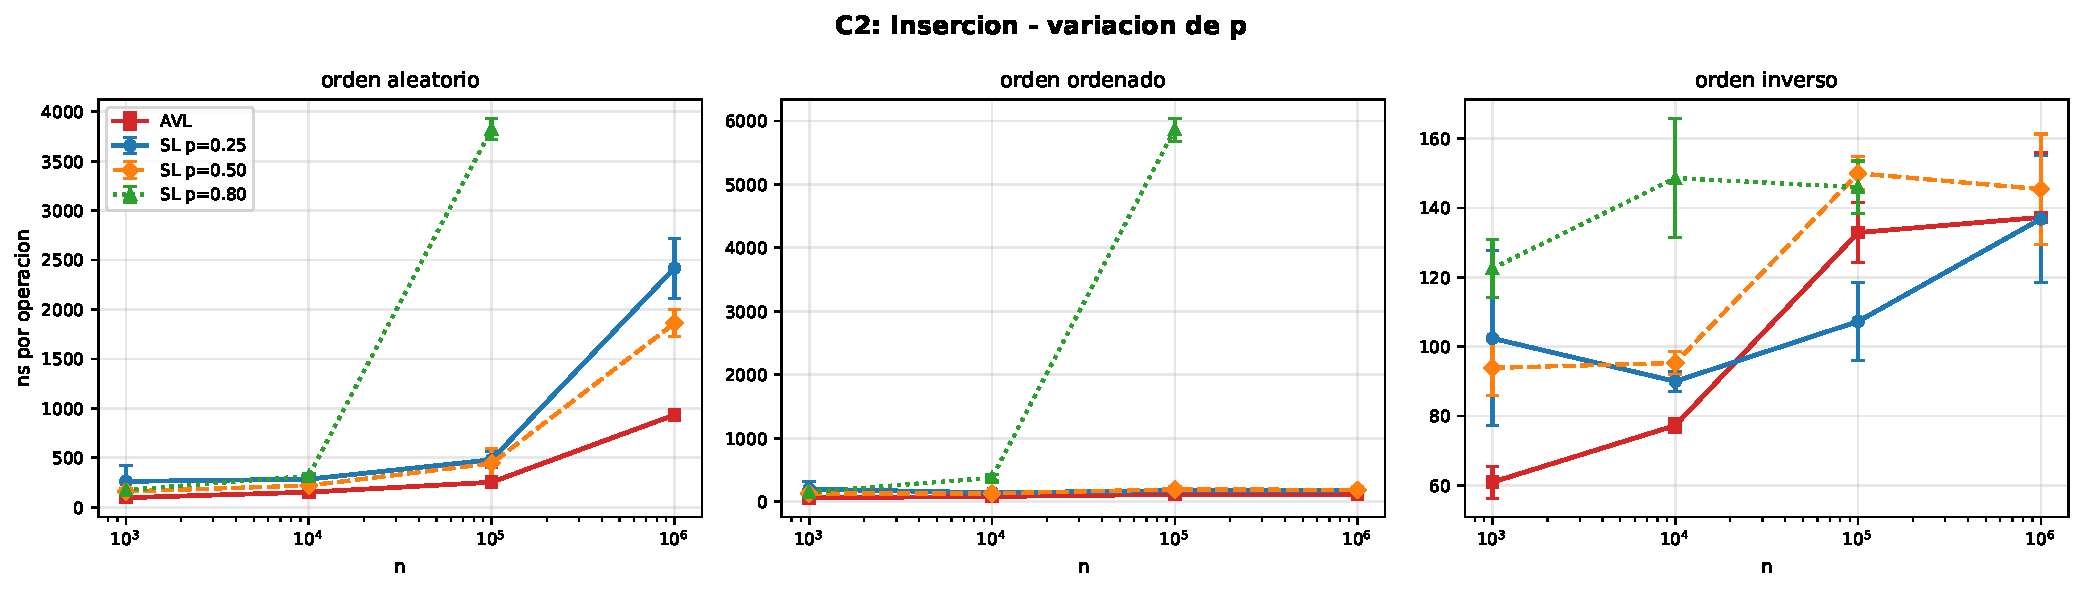
\includegraphics[width=\textwidth]{c2_insert.pdf}
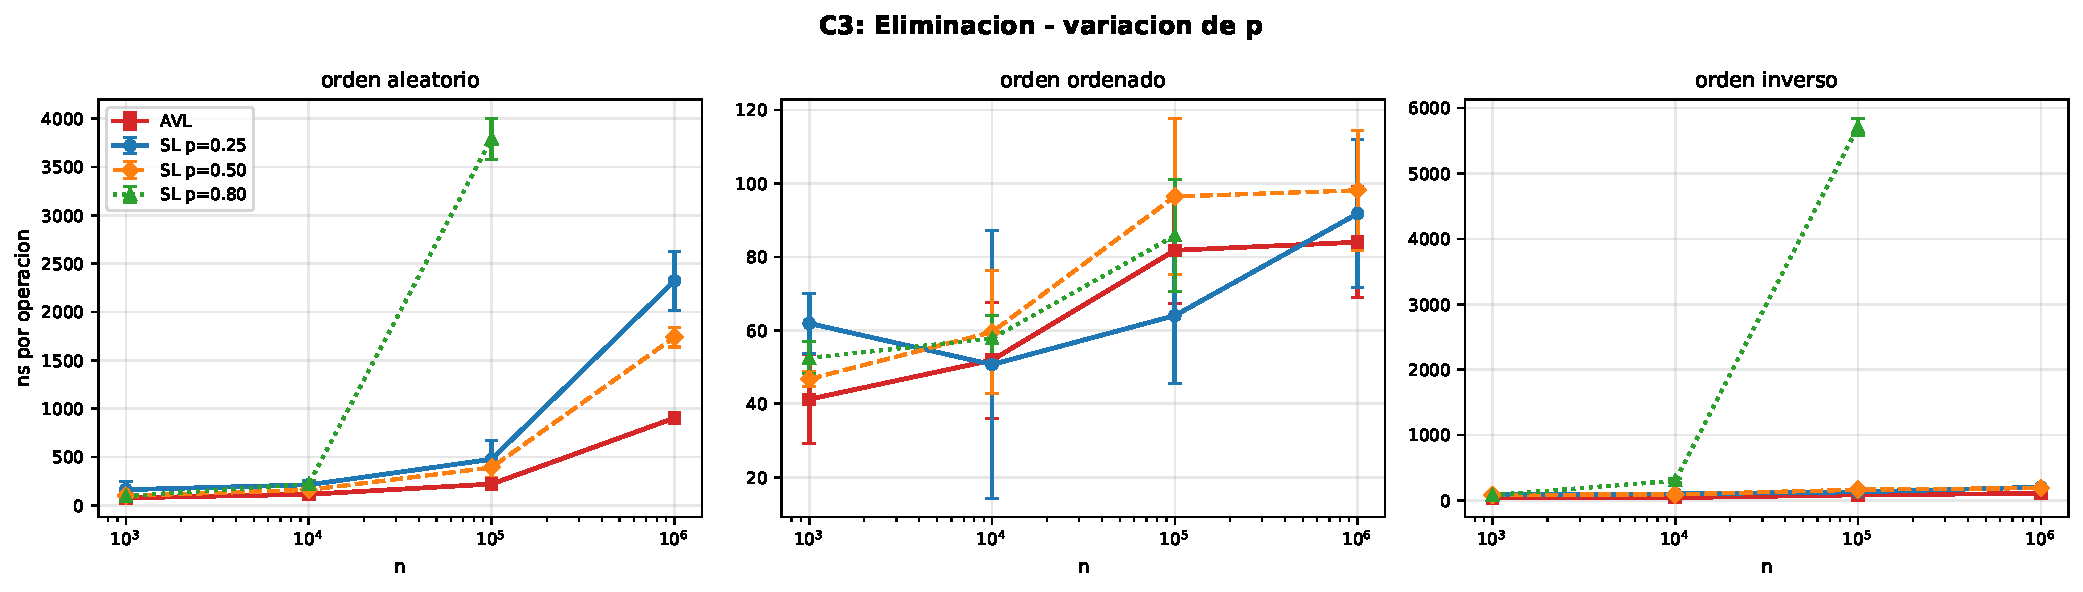
\includegraphics[width=\textwidth]{c3_remove.pdf}
\comando{python scripts/plot\_p\_experiment.py}
\caption{C1--C3: tiempo por operación en función de $n$ para las cuatro
\caption{C1--C3 -- Tiempo por operación en función de $n$ para las cuatro
configuraciones. La Skip List con $p=0.80$ (línea verde punteada) se trunca
en $n=10^5$; su crecimiento es notablemente más rápido que el resto.}
en $n=10^5$ porque su tiempo crece mucho más rápido que el resto.}
\label{fig:c123}
\end{figure}

\begin{figure}[!htb]
\centering
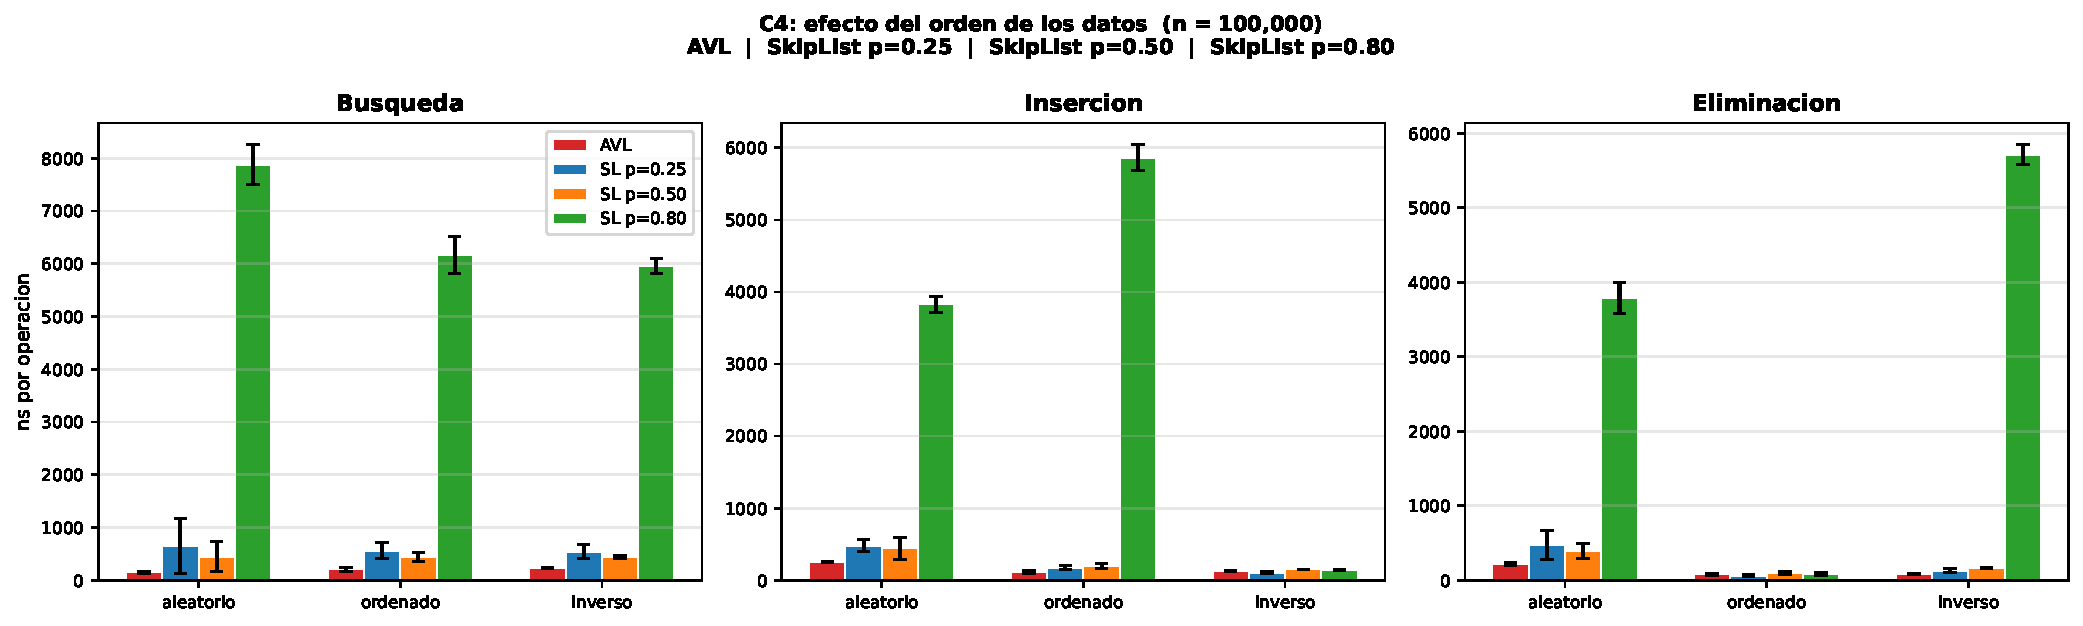
\includegraphics[width=\textwidth]{c4_orden.pdf}
\comando{python scripts/plot\_p\_experiment.py}
\caption{C4: efecto del orden de los datos con $n = 10^5$ para las cuatro
\caption{C4 -- Efecto del orden de los datos con $n = 10^5$ para las cuatro
configuraciones. Las barras de $p=0.80$ dominan en casi todos los escenarios,
salvo inserción inversa y eliminación ordenada.}
\label{fig:c4}
\end{figure}

\paragraph{Análisis e impacto de la caché.}
Los resultados confirman tanto la teoría de Pugh como el peso de la memoria caché:
\begin{itemize}
  \item \textbf{$p=0.25$ frente a $p=0.50$.} Con $p = 0.25$ la Skip List reduce
  casi a la mitad sus niveles (10.7 frente a 19.5 en $n = 10^6$) y usa menos
  punteros por nodo ($1.33$ frente a $2$), pero avanza por más nodos
  horizontales antes de bajar ($\frac{1-p}{p}\log_{1/p} n = 1.5\log_2 n$ nodos
  distintos frente a $1.0\log_2 n$ con $p=0.50$). Cada nodo extra supone un
  posible fallo de caché (agravado por la doble indirección de
  \texttt{std::vector}), lo que explica por qué en datos aleatorios $p=0.25$
  resulta entre $1.2\times$ y $1.5\times$ más lenta que $p=0.50$ ($2748$ frente
  a $1859$\,ns en búsqueda a $n=10^6$). En todos los casos aleatorios el AVL
  mantiene la ventaja porque su nodo cabe en 32\,B contiguos (media línea de
  caché) sin indirecciones adicionales.
Con $p = 0.25$ la Skip List baja casi a la mitad sus niveles (10.7 frente a
19.5 en $n = 10^6$) y guarda menos punteros por nodo ($1.33$ frente a $2$),
pero recorre más nodos horizontales antes de descender
($\frac{1-p}{p}\log_{1/p} n = 1.5\log_2 n$ nodos distintos frente a
$1.0\log_2 n$ con $p=0.50$). Cada nodo adicional puede provocar un fallo de
caché, agravado por la doble indirección de \texttt{std::vector}, por lo que en
datos aleatorios $p=0.25$ fue entre $1.2$ y $1.5$ veces más lenta que $p=0.50$
($2748$ frente a $1859$\,ns en búsqueda con $n=10^6$). Frente a ambas, el AVL
conserva la ventaja porque su nodo ocupa 32\,B contiguos (media línea de caché)
sin indirecciones extra.

  \item \textbf{Colapso de $p=0.80$ a partir de $n=10^4$.} Con $p = 0.80$ cada
  nodo almacena en promedio $1/(1-p) = 5$ punteros (mayor presión sobre la
  caché) y la altura teórica necesaria para $n = 10^5$ sería
  $\log_{1/0.8}(10^5) \approx 52$ niveles. Al estar fijado
  \texttt{MaxLevel}$\,=20$, una fracción $p^{19} = 0.80^{19} \approx 1.44$\,\%
  de los nodos ($\approx 1\,440$ nodos en $n = 10^5$) se acumula en el nivel
  superior, convirtiendo la búsqueda en un recorrido lineal $O(n)$. Con
  $n=10^5$ y datos aleatorios, la búsqueda con $p=0.80$ ($7\,878$\,ns) es
  \textbf{18 veces más lenta} que con $p=0.50$ y \textbf{51 veces más lenta}
  que el AVL.
En cambio, con $p = 0.80$ el rendimiento se degrada a partir de $n = 10^4$.
Cada nodo guarda en promedio $1/(1-p) = 5$ punteros, aumentando la presión
sobre la caché, y la altura teórica necesaria para $n = 10^5$ sería
$\log_{1/0.8}(10^5) \approx 52$ niveles. Como \texttt{MaxLevel} está fijado en
20, una fracción $p^{19} = 0.80^{19} \approx 1.44$\,\% de los nodos
($\approx 1\,440$ nodos en $n = 10^5$) se acumula en el nivel superior y obliga
a recorrerlo casi de forma lineal. En $n=10^5$ con datos aleatorios, la
búsqueda con $p=0.80$ ($7\,878$\,ns) fue 18 veces más lenta que con $p=0.50$ y
51 veces más lenta que el AVL.

  \item \textbf{Casos borde favorables a la Skip List (localidad en cabecera).}
  En \emph{inserción inversa} ($107$\,ns con $p=0.25$ y $146$\,ns con $p=0.80$
  frente a $133$\,ns del AVL) y en \emph{eliminación ordenada} ($64$\,ns con
  $p=0.25$ frente a $82$\,ns del AVL), cada operación inserta o elimina siempre
  la \textbf{clave mínima} del conjunto. En la Skip List ese elemento está
  inmediatamente después de la cabecera (\texttt{head\_}), que permanece
  caliente en caché L1: no realiza saltos horizontales y solo desciende por los
  niveles de \texttt{head\_} ($\approx 9$ niveles con $p=0.25$ frente a
  $\approx 17$ niveles y rebalanceo en el AVL). Esto oculta incluso la
  degeneración de $p=0.80$ en esos dos casos puntuales.
\end{itemize}
Solo en dos escenarios de $n = 10^5$ la Skip List superó al AVL, que fueron
inserción inversa ($107$\,ns con $p=0.25$ y $146$\,ns con $p=0.80$, frente a
$133$\,ns del AVL) y eliminación ordenada ($64$\,ns con $p=0.25$ frente a
$82$\,ns del AVL). En ambos casos cada operación inserta o elimina siempre la
clave mínima del conjunto; en la Skip List esa clave está justo después de la
cabecera (\texttt{head\_}), que permanece en caché L1, así que no hay saltos
horizontales y solo se baja por los niveles de \texttt{head\_} ($\approx 9$
niveles con $p=0.25$ frente a $\approx 17$ niveles y rebalanceo en el AVL). Ese
patrón de acceso incluso oculta la degradación de $p=0.80$ en esos dos casos.

\subsection{Cumplimiento de los objetivos}

La Tabla~\ref{tab:objetivos} resume cómo se cumplió cada objetivo de la
Sección~\ref{sec:plan} y dónde está la evidencia.

\begin{table}[!htb]
\centering
\renewcommand{\arraystretch}{1.2}
\small
\begin{tabularx}{\textwidth}{l >{\raggedright\arraybackslash}X l c}
\toprule
\textbf{Obj.} & \textbf{Evidencia} & \textbf{Dónde} & \textbf{Estado} \\
\midrule
O1 & \texttt{SkipList} según Pugh, con $p$ y \texttt{MaxLevel} configurables & Sec.~\ref{sec:impl}, E1 & Cumplido \\
O2 & \texttt{AvlTree} con rotaciones LL, RR, LR y RL en inserción y eliminación & Sec.~\ref{sec:impl}, E1 & Cumplido \\
O3 & 1\,500\,000 operaciones comparadas con \texttt{std::set} e invariantes, 0 fallos & E1 & Cumplido \\
O4 & \texttt{RandomDatasetGenerator} y \texttt{BenchmarkService}: mismas claves y consultas para ambas estructuras & Sec.~\ref{sec:metodo} & Cumplido \\
O4 & \texttt{RandomDatasetGenerator} y \texttt{BenchmarkService} aplican las mismas claves y consultas a ambas estructuras & Sec.~\ref{sec:metodo} & Cumplido \\
O5 & 12 escenarios $\times$ 10 repeticiones, gráficos G1--G4 y C1--C4, análisis teórico y variación de $p \in \{0.25, 0.50, 0.80\}$ & E2, E3, E4 & Cumplido \\
\bottomrule
\end{tabularx}
\caption{Cumplimiento de los objetivos específicos.}
\label{tab:objetivos}
\end{table}

% ============================================================
\section{Plan de trabajo}\label{sec:cronograma}

El proyecto va de la semana 9 a la 15 del ciclo. En la semana 9 se entrega
esta propuesta, las semanas 10 a 14 son las cinco semanas de desarrollo y la
semana 15 corresponde a la exposición final. La Tabla~\ref{tab:cronograma}
muestra cómo repartimos el trabajo y el resultado que esperamos tener al final
de cada semana.
El proyecto abarcó de la semana 9 a la 15 del ciclo. En la semana 9 se entregó
la propuesta, entre las semanas 10 y 14 se realizó el desarrollo y la
evaluación experimental, y la semana 15 corresponde a la exposición final. La
Tabla~\ref{tab:cronograma} muestra la distribución del trabajo y el resultado
obtenido al final de cada semana.

\begin{table}[!htb]
\centering
\renewcommand{\arraystretch}{1.25}
\small
\setlength{\tabcolsep}{4pt}
\begin{tabular}{>{\raggedright\arraybackslash}p{4.7cm}*{7}{>{\centering\arraybackslash}p{0.62cm}}>{\raggedright\arraybackslash}p{4.4cm}}
\toprule
\textbf{Actividad} & \textbf{S9} & \textbf{S10} & \textbf{S11} & \textbf{S12} & \textbf{S13} & \textbf{S14} & \textbf{S15} & \textbf{Resultado} \\
\midrule
Propuesta del proyecto            & \on & & & & & & & Propuesta entregada \\
Revisión bibliográfica y diseño   & & \on & & & & & & Interfaces y plan de pruebas \\
Implementación del código         & & & \on & & & & & Código de ambas estructuras \\
Pruebas y datos de prueba         & & & & \on & & & & Pruebas y generador listos \\
Experimentos y medición           & & & & & \on & & & Tiempos de los 12 escenarios \\
Análisis, gráficos y redacción    & & & & & & \on & & Gráficos G1--G4 e informe \\
Análisis, gráficos y redacción    & & & & & & \on & & Gráficos G1--G4, C1--C4 e informe \\
Exposición final                  & & & & & & & \on & Presentación \\
\bottomrule
\end{tabular}
\caption{Cronograma seguido por semana del ciclo (S = semana).}
\label{tab:cronograma}
\end{table}

% ============================================================
\section{Conclusiones}\label{sec:conclusiones}

\begin{itemize}
  \item Cumplimos los objetivos O1--O5: implementamos ambas estructuras desde
  \item Cumplimos los objetivos O1--O5; implementamos ambas estructuras desde
  cero, las verificamos contra \texttt{std::set}, construimos el generador y
  el programa de medición, y obtuvimos los gráficos G1--G4.
  el programa de medición, y obtuvimos los gráficos G1--G4 y C1--C4.
  \item \textbf{P1.} Ambas estructuras crecen de forma logarítmica mientras
  caben en caché, y bastante más rápido después. En nuestra implementación el
  AVL fue más rápido en todas las operaciones y tamaños, entre 1.1 y 2.9 veces,
  y la ventaja aumentó con $n$.
  \item \textbf{P2.} El orden de los datos influyó más que la estructura:
  caben en caché, y bastante más rápido después. En nuestra implementación con
  $p = 1/2$, el AVL fue más rápido en todas las operaciones y tamaños, entre
  1.1 y 2.9 veces, y la ventaja aumentó con $n$.
  \item \textbf{P2.} El orden de los datos influyó más que la estructura;
  insertar y eliminar claves ordenadas fue hasta 10 veces más rápido que
  hacerlo al azar en ambas. La forma de la skip list no dependió del orden,
  como predice la teoría; la del AVL sí, aunque siempre quedó balanceado.
  \item \textbf{P3.} El parámetro $p$ resulta crítico: con \texttt{MaxLevel}$\,=20$,
  $p=0.80$ degenera a partir de $n \approx 10^4$ y llega a ser 51 veces más
  lenta que el AVL en búsqueda aleatoria a $n=10^5$. Entre $p=0.50$ y $p=0.25$,
  $p=0.50$ es más rápida en datos aleatorios, mientras $p=0.25$ ahorra niveles
  y memoria a costa de un 20--50\,\% más de tiempo por mayor número de nodos
  visitados y fallos de caché.
  \item La misma complejidad asintótica no implica el mismo rendimiento: el
  \item \textbf{P3.} El parámetro $p$ influye de forma marcada; con
  \texttt{MaxLevel}$\,=20$, $p=0.80$ degenera desde $n \approx 10^4$ y llega a
  ser 51 veces más lenta que el AVL en búsqueda aleatoria a $n=10^5$. Entre
  $p=0.50$ y $p=0.25$, $p=0.50$ rinde mejor en datos aleatorios, mientras que
  $p=0.25$ ahorra niveles y memoria a costa de un 20--50\,\% más de tiempo por
  el mayor número de nodos visitados y fallos de caché.
  \item La misma complejidad asintótica no implica el mismo rendimiento; el
  número de nodos visitados y el acceso a memoria explican la diferencia. La
  principal ventaja práctica de la skip list (su facilidad para versiones
  concurrentes, como en Redis o RocksDB) no se mide en este experimento
  secuencial.
\end{itemize}

\paragraph{Limitaciones y trabajo futuro.}
Todas las mediciones se hicieron en una sola máquina y con un solo
compilador. Una skip list con los punteros integrados en el mismo bloque de
memoria que el nodo (eliminando la doble indirección de \texttt{std::vector})
o con un asignador de memoria contiguo reduciría la brecha frente al AVL; esa
variante se puede probar con el código actual agregando una nueva fábrica sin
modificar el núcleo del benchmark.
compilador. Una skip list con los punteros dentro del mismo bloque de memoria
que el nodo (sin la doble indirección de \texttt{std::vector}) o con un
asignador contiguo reduciría la diferencia frente al AVL; esa variante se puede
probar con el código actual agregando una nueva fábrica sin tocar el núcleo del
benchmark.

\paragraph{Reproducibilidad.}
El código, las pruebas, los resultados en CSV y los scripts de gráficos están
en el repositorio del proyecto. Para repetir todo:
\begin{itemize}[leftmargin=1.4em, itemsep=1pt, topsep=2pt]
  \item Compilación y correctitud (E1): \texttt{./build.sh} y \texttt{./build/correctness\_tests}.
  \item Benchmarks (E2--E4): \texttt{./build/benchmark -{}-out results},
  \texttt{./build/benchmark -{}-p 0.25 -{}-out results/p025} y
  \texttt{./build/benchmark -{}-p 0.80 -{}-sizes 1000,10000,100000 -{}-out results/p080}.
  \item Gráficos: \texttt{python scripts/plot\_results.py},
  \texttt{python scripts/plot\_extra.py} y \texttt{python scripts/plot\_p\_experiment.py}.
\end{itemize}
en el repositorio del proyecto. Para repetir el estudio completo basta ejecutar
\texttt{./build.sh} y \texttt{./build/correctness\_tests}, correr
\texttt{./build/benchmark} con \texttt{-{}-out results}, con
\texttt{-{}-p 0.25} \texttt{-{}-out results/p025} y con
\texttt{-{}-p 0.80} \texttt{-{}-sizes 1000,10000,100000}
\texttt{-{}-out results/p080}, y generar las figuras con
\texttt{scripts/plot\_results.py}, \texttt{scripts/plot\_extra.py} y
\texttt{scripts/plot\_p\_experiment.py}.

% ============================================================
\begin{thebibliography}{9}
\small
\setlength{\itemsep}{1pt}

\bibitem{pugh1990}
W.~Pugh.
\newblock Skip lists: A probabilistic alternative to balanced trees.
\newblock \emph{Communications of the ACM}, 33(6):668--676, 1990.
\newblock \url{https://doi.org/10.1145/78973.78977}

\bibitem{vadrevu2024}
L.~Xing, V.~S.~P.~K.~Vadrevu y W.~G.~Aref.
\newblock The ubiquitous skiplist: A survey of what cannot be skipped about the
skiplist and its applications in data systems.
\newblock \emph{ACM Computing Surveys}, 57(11):1--37, 2025.
\newblock \url{https://doi.org/10.1145/3736754}

\bibitem{avl1962}
G.~M.~Adel'son-Vel'skii y E.~M.~Landis.
\newblock An algorithm for the organization of information.
\newblock \emph{Soviet Mathematics Doklady}, 3:1259--1263, 1962.

\bibitem{knuth1998}
D.~E.~Knuth.
\newblock \emph{The Art of Computer Programming, Vol.~3: Sorting and
Searching}, 2.\textsuperscript{a} ed.
\newblock Addison-Wesley, 1998.

\bibitem{munro1992}
J.~I.~Munro, T.~Papadakis y R.~Sedgewick.
\newblock Deterministic skip lists.
\newblock En \emph{Proceedings of the Third Annual ACM-SIAM Symposium on
Discrete Algorithms (SODA)}, pp.~367--375, 1992.

\end{thebibliography}

\end{document}
